\documentclass[a4paper, 10pt]{article}

\usepackage[utf8]{inputenc}
\usepackage[english]{babel}
\usepackage[T1]{fontenc}
\usepackage{lmodern}
\usepackage[width=15.50cm, height=22.00cm]{geometry}
\usepackage{amsmath}
\usepackage{amssymb}
\usepackage{amsthm}
\usepackage{esdiff}
\usepackage{url}
\usepackage{listings}
\usepackage{color}
\usepackage{graphicx}
\usepackage{subcaption}
\usepackage{caption}

\definecolor{mygreen}{rgb}{0,0.6,0}
\definecolor{mygray}{rgb}{0.5,0.5,0.5}
\definecolor{light}{rgb}{0.96, 0.96, 0.96}
\definecolor{mymauve}{rgb}{0.58,0,0.82}

\lstset{ %
	backgroundcolor=\color{light},   % choose the background color; you must add \usepackage{color} or \usepackage{xcolor}
	basicstyle=\footnotesize,        % the size of the fonts that are used for the code
	breakatwhitespace=false,         % sets if automatic breaks should only happen at whitespace
	breaklines=true,                 % sets automatic line breaking
	captionpos=b,                    % sets the caption-position to bottom
	commentstyle=\color{mygreen},    % comment style
	deletekeywords={},            	 % if you want to delete keywords from the given language
	escapeinside={\%*}{*)},          % if you want to add LaTeX within your code
	extendedchars=true,              % lets you use non-ASCII characters; for 8-bits encodings only, does not work with UTF-8
	frame=single,	                 % adds a frame around the code
	keepspaces=true,                 % keeps spaces in text, useful for keeping indentation of code (possibly needs columns=flexible)
	keywordstyle=\color{blue},       % keyword style
	language=C++,                    % the language of the code
	otherkeywords={},           	 % if you want to add more keywords to the set
	numbers=left,                    % where to put the line-numbers; possible values are (none, left, right)
	numbersep=5pt,                   % how far the line-numbers are from the code
	numberstyle=\tiny\color{mygray}, % the style that is used for the line-numbers
	rulecolor=\color{black},         % if not set, the frame-color may be changed on line-breaks within not-black text (e.g. comments (green here))
	showspaces=false,                % show spaces everywhere adding particular underscores; it overrides 'showstringspaces'
	showstringspaces=false,          % underline spaces within strings only
	showtabs=false,                  % show tabs within strings adding particular underscores
	stepnumber=1,                    % the step between two line-numbers. If it's 1, each line will be numbered
	stringstyle=\color{mymauve},     % string literal style
	tabsize=3,	                     % sets default tabsize to 2 spaces
	title=\lstname                   % show the filename of files included with \lstinputlisting; also try caption instead of title
}

\setlength{\parindent}{1 cm}
\setlength{\parskip}{0 cm}
\pagenumbering{arabic}
\frenchspacing
\selectlanguage{english}

\newtheorem{mydef}{Definition}
\newcommand{\horrule}[1]{\rule{\linewidth}{#1}}
\newcommand{\includecode}[2][c]{\lstinputlisting[caption=#2, escapechar=, style=custom#1]{#2}<!---->}
\newcommand{\norm}[1]{\lVert#1\rVert}
\newcommand{\abs}[1]{\lvert#1\rvert}
\renewcommand{\vec}[1]{\mathbf{#1}}

\title{\horrule{0.5 pt}\\[0.4cm] \textbf{Weather Data Visualization} \horrule{1 pt}}
\author{Petr Valenta}
\date{\today}

\begin{document}

\maketitle
{\small This document is a part of the assessment work for the subject WMMS535V Scientific Visualization lectured at ENSIMAG, Grenoble INP.}

\begin{abstract}
This document describes a C++ code which has been used to compute colormaps and isocontours from provided weather data and to export them in order to visualize a results in Google Earth. One can find explanation of individual steps of the implementation and used data structures. Furthermore, the Hardy multiquadrics and the Shepard's method used for the interpolation of the scattered data on the uniform grid are briefly discussed. Finally, there are presented the results of this work. All source files can be found at \url{http://kfe.fjfi.cvut.cz/~valenpe7/files/INP/scientific_visualization}.
\end{abstract}

\tableofcontents

\section{Introduction}
The goal of this project was to visualize data from Meteo France in Google Earth, using several methods presented in the lecture. Meteo France provides publicly available data recording wind velocities, temperatures and pressures at several cities. The work consists in the following four main steps:
\begin{enumerate}
	\setlength{\itemsep}{0cm}%
	\item read and import the scattered data
	\item interpolate the scattered data in order to evaluate data at arbitrary positions, using the Shepard's method and the Hardy multiquadrics
	\item compute colormap images and isocontours from the interpolated data
	\item export the colormap images and the isocontours in a KML (Keyhole Markup Language) format file in order to visualize the data in Google Earth
\end{enumerate}
The project has been carried out using C++ language. In the next section one can find a description of individual steps of the implementation which leads to the final visualization.

\section{Implementation}
The main idea how to deal with several steps of implementation was to make only one class for the data processing, which includes data structures for scattered and uniform data as well as all methods beginning with the input data loading and ending with the required visualization. One can find the listings of this class below, individual methods and data structures will be described later.
\begin{lstlisting}[caption=main class for weather data processing]
class weather_data {
public:
	weather_data();
	void load_data(std::string input_file);
	void create_grid(std::array<unsigned int, 2> size);
	weather_data& shepard_interpolation(double p);
	weather_data& hardy_interpolation(double R);
	weather_data& compute_colormap(std::vector<std::array<int, 4>> color_table);
	weather_data& compute_isolines(unsigned int n);
	void export_colormap();
	void export_isolines();
	~weather_data();
private:
	std::string name;
	uniform_data uniform;
	scattered_data scattered;
	std::vector<unsigned char> colormap;
	std::vector<isoline> isolines;
};
\end{lstlisting}

The main advantage of this approach is simpler and faster way to access the data during the interpolation of scattered data on the uniform grid. The drawback is obviously inability to use the code for solving another similar problems as well as its more demanding extensibility. 

\subsection{Loading input data}
The first step is to gather and parse the data. Meteo France provides publicly available data including atmospheric parameters measured or observed at the several France meteorological stations in the CSV (Comma-Separated Values) file format. For the purposes of the project, we are interested in temperature, atmospheric pressure and wind velocity. Since all the data undergo the same process before the final visualization, the data are loaded from separate CSV files, which have to contain three columns. The first two are dedicated for latitude and longitude of the site and the last one for the value of the measured parameter.

Scattered data are parsed into the following data structure: 
\begin{lstlisting}[caption=data structure for scattered data]
typedef struct {
	unsigned int size;
	std::array<double, 4> boundary;
	std::vector<std::array<double, 3>> values;
} scattered_data;
\end{lstlisting}
The "size" value stands for the number of the rows in the input file (number of the stations), the "boundary" saves minimal and maximal coordinates, and the array of three vectors "values" is dedicated for the data itself.

The responsibility for the data loading takes the following method:
\begin{lstlisting}[caption=method for parsing the data]
void weather_data::load_data(std::string filename) {
	std::ifstream input_file;
	std::string line;
	std::cout << "loading scattered data: " << filename << std::endl;
	this->name = filename.substr(0, filename.find_last_of("."));
	input_file.open(filename);
	if(input_file.fail()) {
		std::cerr << "error: cannot read input file" << std::endl;
		return;
	}
	this->scattered.size = 0;
	while(std::getline(input_file, line)) {
		++this->scattered.size;
	}
	input_file.clear();
	input_file.seekg(0, std::ios::beg);
	this->scattered.values.resize(this->scattered.size);
	if(input_file.is_open()) {
		for(std::size_t i = 0; i < this->scattered.size; ++i) {
			for(std::size_t j = 0; j < 3; ++j) {
				input_file >> this->scattered.values[i][j];
				input_file.get();
			}
		}
	}
	double min_x = this->scattered.values[0][0];
	double max_x = this->scattered.values[0][0];
	double min_y = this->scattered.values[0][1];
	double max_y = this->scattered.values[0][1];
	for(std::size_t i = 0; i < this->scattered.size; ++i) {
		min_x = std::min(min_x, this->scattered.values[i][0]);
		max_x = std::max(max_x, this->scattered.values[i][0]);
		min_y = std::min(min_y, this->scattered.values[i][1]);
		max_y = std::max(max_y, this->scattered.values[i][1]);
	}
	this->scattered.boundary = {min_x, max_x, min_y, max_y};
	std::cout << "scattered data loaded successfully" << std::endl;
	return;
}
\end{lstlisting}
This method reads and imports the data from a given file and keeps the name of the file, number of rows and boundaries. 

\subsection{Creating uniform grid}
Since the input data are loaded, we need to create a two dimensional uniform grid to be able to perform interpolation. Similarly as before, we need a data structure for uniform data:
\begin{lstlisting}[caption=data structure for uniform data]
typedef struct {
	std::array<unsigned int, 2> size;
	std::array<double, 2> spacing;
	std::array<double, 4> boundary;
	std::vector<std::vector<cell>> cells;
	std::vector<std::vector<node>> nodes;
} uniform_data;
\end{lstlisting}
This data structure contains the size of the grid, which is now pair of integers (number of nodes in x and y direction), spacing between two nodes in both directions, minimal and maximal coordinates, the matrix of cells and the matrix of nodes.

The matrices of cells and nodes use a special data types. The first data type is 
cell:
\begin{lstlisting}[caption=class cell]
class cell {
	friend class weather_data;
public:
	cell() = default;
	segment top_bottom();
	segment top_left();
	segment top_right();
	segment bottom_left();
	segment bottom_right();
	segment left_right();
	cell& compute_average();
	~cell() = default;
private:
	int id;
	double average;
	std::array<int, 4> RGBA;
	std::array<node*, 4> nodes;
};
\end{lstlisting}
This class contains id, four pointers to the nodes assigned to the cell, average of the values, which will be interpolated into these nodes and RGBA color space, which will take a value according to the average in order to compute colormap.

Moreover, this class includes the method for computing the average value of nodes assigned to the cell as well as several methods for selecting a segment of this cell in order to compute isolines. The segment data structure contains only coordinates of the starting and ending points:
\begin{lstlisting}[caption=class segment]
class segment {
	friend class cell;
	friend class weather_data;
public:
	segment() = default;
	~segment() = default;
private:
	std::array<double, 2> start;
	std::array<double, 2> end;
};
\end{lstlisting}

The second data type is used to describe a nodes. This class is significantly simpler than the cell class, it contains only id and three floating point numbers: latitude, longitude and the value of measured parameter. 
\begin{lstlisting}[caption=class node]
class node {
	friend class cell;
	friend class weather_data;
public:
	node() = default;
	~node() = default;
private:
	int id;
	std::array<double, 3> values;
};
\end{lstlisting}

The second step in the data processing pipeline is to create a two dimensional uniform grid. For this purpose, there is a method in the main class:
\begin{lstlisting}[caption= method for creating uniform grid]
void weather_data::create_grid(std::array<unsigned int, 2> size) {
	if(!size[0] || !size[1]) {
		std::cerr << "error: cannot create grid" << std::endl;
		return;
	}
	std::cout << "creating uniform grid of size: " << size[0] << " x " << size[1] << std::endl;
	this->uniform.size = {
		size[0],
		size[1]
	};
	this->uniform.boundary = this->scattered.boundary;
	this->uniform.spacing = {
		(this->uniform.boundary[1] - this->uniform.boundary[0]) / this->uniform.size[0],
		(this->uniform.boundary[3] - this->uniform.boundary[2]) / this->uniform.size[1]
	};
	this->uniform.nodes.resize(this->uniform.size[1]);
	for(std::size_t i = 0; i < this->uniform.size[1]; ++i) {
		this->uniform.nodes[i].resize(this->uniform.size[0]);
	}
	for(std::size_t i = 0; i < this->uniform.size[1]; ++i) {
		for(std::size_t j = 0; j < this->uniform.size[0]; ++j) {
			this->uniform.nodes[i][j].id = this->uniform.size[0] * i + j;
			this->uniform.nodes[i][j].values[0] = this->uniform.boundary[0] + j * this->uniform.spacing[0];
			this->uniform.nodes[i][j].values[1] = this->uniform.boundary[2] + i * this->uniform.spacing[1];
			this->uniform.nodes[i][j].values[2] = 0.0;
		}
	}
	this->uniform.cells.resize(this->uniform.size[1] - 1);
	for(std::size_t i = 0; i < this->uniform.size[1] - 1; ++i) {
		this->uniform.cells[i].resize(this->uniform.size[0] - 1);
	}
	for(std::size_t i = 0; i < this->uniform.size[1] - 1; ++i) {
		for(std::size_t j = 0; j < this->uniform.size[0] - 1; ++j) {
			this->uniform.cells[i][j].id = (this->uniform.size[0] - 1) * i + j;
			this->uniform.cells[i][j].average = 0.0;
			this->uniform.cells[i][j].RGBA = {0, 0, 0, 255};
			this->uniform.cells[i][j].nodes = {
				&this->uniform.nodes[i][j],
				&this->uniform.nodes[i][j + 1],
				&this->uniform.nodes[i + 1][j + 1],
				&this->uniform.nodes[i + 1][j],
			};
		}
	}
	std::cout << "uniform grid created successfully" << std::endl;
	return;
}
\end{lstlisting}
This method takes the size of the grid in both directions as an argument. This value significantly influences the quality and the computational time of the interpolation as well as the resolution of the computed colormap and the smoothness of the isolines. The location of the grid is done automatically in accordance with the boundaries of the scattered data. This method also initializes the fields of cells and nodes.

\subsection{Performing interpolation}
The crucial step is the interpolation of scattered data in order to evaluate measured parameters at the grid points. In accordance with the project specifications, two following methods have been used.
\subsubsection*{Shepard's method}
The principle of finding an interpolated value of scattered data $ f_{i} = f\left( \vec{x}_{i} \right) $ for $ i \in \left\lbrace 1, \ldots, N \right\rbrace $ at a given point $ \vec{x} $ using Shepard's method, is based on constructing an interpolating function $ F\left( \vec{x} \right) $
\begin{equation}
F \left( \vec{x} \right) = \sum_{i = 1}^{N} \omega_{i} \left( \vec{x} \right) f_{i},
\end{equation}
where the weighting function $ \omega_{i} \left( \vec{x} \right) $ is defined by Shepard as follows \cite{shepard},
\begin{equation}
\omega_{i} \left( \vec{x} \right) = \frac{1}{\mathrm{d} \left( \vec{x}, \: \vec{x}_{i}\right) ^{p}} \cdot \frac{1}{\sum \limits_{j = 1}^{N} \frac{1}{\mathrm{d} \left( \vec{x}, \: \vec{x}_{j}\right) ^{p}}}, \qquad \mathrm{d}\left( \vec{x}, \: \vec{x}_{i} \right) = \lVert \vec{x} - \vec{x}_{i} \rVert
\end{equation}
and $ p $ is a positive real number, called the power parameter.

The implementation of this method is attached below. In the first step, the weighting function $ \omega_{i} \left( \vec{x} \right) $ is computed for each grid point. Afterwards, the measured parameter is evaluated there.
\begin{lstlisting}[caption = implementation of Shepard's method]
weather_data& weather_data::shepard_interpolation(double p) {
	std::cout << "performing interpolation using the sheppard method with parameter p = " << p << std::endl;
	std::vector<std::vector<double>> w;
	w.resize(this->uniform.size[1]);
	for(std::size_t i = 0; i < this->uniform.size[1]; ++i) {
		w[i].resize(this->uniform.size[0]);
	}
	for(std::size_t i = 0; i < this->uniform.size[1]; ++i) {
		for(std::size_t j = 0; j < this->uniform.size[0]; ++j) {
			w[i][j] = 0.0;
			this->uniform.nodes[i][j].values[2] = 0.0;
			for(std::size_t k = 0; k < this->scattered.size; ++k) {
				w[i][j] += 1.0 / pow(sqrt(pow(this->uniform.nodes[i][j].values[0] - this->scattered.values[k][0], 2)
				+ pow(this->uniform.nodes[i][j].values[1] - this->scattered.values[k][1], 2)), p);
			}
			for(std::size_t k = 0; k < this->scattered.size; ++k) {
				this->uniform.nodes[i][j].values[2] += (1.0 / pow(sqrt(pow(this->uniform.nodes[i][j].values[0]
				- this->scattered.values[k][0], 2) + pow(this->uniform.nodes[i][j].values[1]
				- this->scattered.values[k][1], 2)), p)) * (1.0 / w[i][j]) * this->scattered.values[k][2];
			}
		}
	}
	std::cout << "scattered data successfully interpolated to uniform grid" << std::endl;
	return (*this);
}
\end{lstlisting}

\subsubsection*{Hardy multiquadrics}
The second method, which has been implemented, is called Hardy multiquadrics. Now, we are looking for the interpolating function in the following form \cite{hardy},
\begin{equation}
F\left( \vec{x} \right) = \sum_{i = 1}^{N} \alpha_{i} h_{i} \left( \vec{x} \right), 
\end{equation}
where $ \alpha_{i} $ are unknown coefficients and
\begin{equation}
h_{i} \left( \vec{x} \right) = \sqrt{R + \mathrm{d} \left( \vec{x}, \: \vec{x}_{i} \right)^{2} }.
\end{equation}
The input argument R is a nonzero shape parameter. The coefficients $ \alpha_{i} $ are calculated by solving the system of equations given by the conditions
\begin{equation}
F\left( \vec{x}_{i} \right) = f_{i}.
\end{equation}
It was proved \cite{micchelli} that for distinct data, this system of equations is always solvable.

The implementation of the Hardy's method has been carried out as follows, 
\begin{lstlisting}[caption = implementation of Hardy multiquadrics]
weather_data& weather_data::hardy_interpolation(double R) {
	std::cout << "performing interpolation using the hardy multiquadrics with parameter R = " << R << std::endl;
	Eigen::MatrixXd b(this->scattered.size, this->scattered.size);
	Eigen::VectorXd alpha(this->scattered.size);
	Eigen::VectorXd f(this->scattered.size);
	for(std::size_t k = 0; k < this->scattered.size; ++k) {
		f(k) = this->scattered.values[k][2];
		for(std::size_t l = 0; l < this->scattered.size; ++l) {
			b(k, l) = sqrt(R + pow(this->scattered.values[k][0] - this->scattered.values[l][0], 2)
			+ pow(this->scattered.values[k][1] - this->scattered.values[l][1], 2));
		}
	}
	alpha = b.lu().solve(f);
	std::vector<double> h;
	h.resize(this->scattered.size);
	for(std::size_t i = 0; i < this->uniform.size[1]; ++i) {
		for(std::size_t j = 0; j < this->uniform.size[0]; ++j) {
			this->uniform.nodes[i][j].values[2] = 0.0;
			for(std::size_t k = 0; k < this->scattered.size; ++k) {
				h[k] = sqrt(R + pow(this->uniform.nodes[i][j].values[0] - this->scattered.values[k][0], 2)
				+ pow(this->uniform.nodes[i][j].values[1] - this->scattered.values[k][1], 2));
				this->uniform.nodes[i][j].values[2] += alpha(k) * h[k];
			}
		}
	}
	std::cout << "scattered data successfully interpolated to uniform grid" << std::endl;
	return (*this);
}
\end{lstlisting}
The system of linear equations is solved using LU decomposition from the Eigen C++ library. Then the function $ h_{i} \left( \vec{x} \right) $ is computed at each grid point and the measured parameter is evaluated there.

\subsection{Computing colormap}
Since we have interpolated values of measured parameter at each grid point, one is able to compute a colormap. The idea is to calculate an average value of the four nodes assigned to each cell. Then the maximum and minimum of all average values are determined and the interval, which these two numbers form, is divided into several parts corresponding to the number of colors in used color table. Afterwards, each cell will get the RGB value from the color table according to its average value. The implementation have been done as follows.   
\begin{lstlisting}[caption = method for computing a colormap]
weather_data& weather_data::compute_colormap(std::vector<std::array<int, 4>> color_table) {
	std::cout << "computing colormap.. " << std::endl;
	double max = 0.0;
	double min = std::numeric_limits<double>::infinity();
	for(std::size_t i = 0; i < this->uniform.size[1] - 1; ++i) {
		for(std::size_t j = 0; j < this->uniform.size[0] - 1; ++j) {
			this->uniform.cells[i][j].compute_average();
			max = std::max(max, this->uniform.cells[i][j].average);
			min = std::min(min, this->uniform.cells[i][j].average);
		}
	}
	unsigned int n = color_table.size();
	double span = (max - min) / n;
	std::cout << "number of colors: " << n << std::endl;
	this->colormap.resize((this->uniform.size[0] - 1) * (this->uniform.size[1] - 1) * 4);
	for(std::size_t i = 0; i < this->uniform.size[1] - 1; ++i) {
		for(std::size_t j = 0; j < this->uniform.size[0] - 1; ++j) {
			for(std::size_t k = 0; k < n; ++k) {
				if(this->uniform.cells[i][j].average <= min + (k + 1) * span && this->uniform.cells[i][j].average >= min + k * span) {
					this->uniform.cells[i][j].RGBA = color_table[k];
				}
			}
			for(std::size_t k = 0; k < 4; ++k) {
				this->colormap[4 * ((this->uniform.size[1] - i - 2) * (this->uniform.size[0] - 1) + j) + k] = this->uniform.cells[i][j].RGBA[k];
			}
		}
	}
	std::cout << "colormap created successfully" << std::endl;
	return (*this);
}
\end{lstlisting}

\subsection{Computing isolines}
Similarly as before, the method for computing isolines takes a number of isolines as an argument. Then the maximal and minimal value assigned to each grid point is calculated, and the interval, which these two numbers form, is divided by the number of isolines, we want to get. The isolines are computed in accordance with these thresholds using so called marching squares algorithm. The implementation is quite lengthy, therefore it is not attached to this document. Nevertheless, one can find it in the code.

\subsection{Exporting data}
In order to visualize the data, we have computed before, in Google Earth, it is necessary to export them in KML file format. For the colormap, first we need to export the generated image in PNG format. For this reason, the LodePNG C++ library has been used. Then we need to generate a KML file with the specified path to the colormap image and the coordinates, where this image should appear. This coordinates are determined by boundaries we computed before. For the isolines, we need to export separate lines determined by its starting and ending points. These lines we computed before as a segments. In a result, they will create a whole isoline.

There exists a KML library written in C++ called libkml, but it is deprecated. Thus, I decided to write own methods for exporting the data into a KML file. The implementation is not difficult, but a little bit long. One can find it in a code. 

\section{Compilation and executing}
Before the compilation, several settings have to be done. By default, the size of grid is set to 1025 nodes in both directions, which leads to the size of generated colormap 1024 x 1024. Then the Shepard's interpolation with parameter $ p = 2 $ is performed. For the colormap, the predefined color table jet with 64 colors is used. After that, 6 isolines are computed, and both, colormap and isolines, are exported to the KML file. 

One can change the arguments, uncomment one of the methods for interpolation, but the order of the following data processing pipeline has to be kept.
\begin{lstlisting}[caption = data processing pipeline]
void run_visualization(std::string input_file) {
	weather_data quantity;
	quantity.load_data(input_file);
	quantity.create_grid({1025, 1025});
	quantity.shepard_interpolation(2.0);
	//quantity.hardy_interpolation(2.0);
	quantity.compute_colormap(jet);
	quantity.compute_isolines(6);
	quantity.export_colormap();
	quantity.export_isolines();
	return;
}
\end{lstlisting}

For the compilation, one can use the attached bash script "compile" which executes prepared makefile. Due to the usage of features introduced by the latest revision of C++ standards, the minimum required version of GCC is 4.8.

Compiled application takes the filename of the input data as an argument. Both, the application and the input file, have to be located in the same directory. 

\section{Results}
In the last section, the results are presented. Several test visualizations have been done in Google Earth to verify the correctness of the code output. One can find two examples in the figures 1 and 2.

\begin{figure}[!htb]
	\centering
	\begin{minipage}{.5\textwidth}	
		\centering
		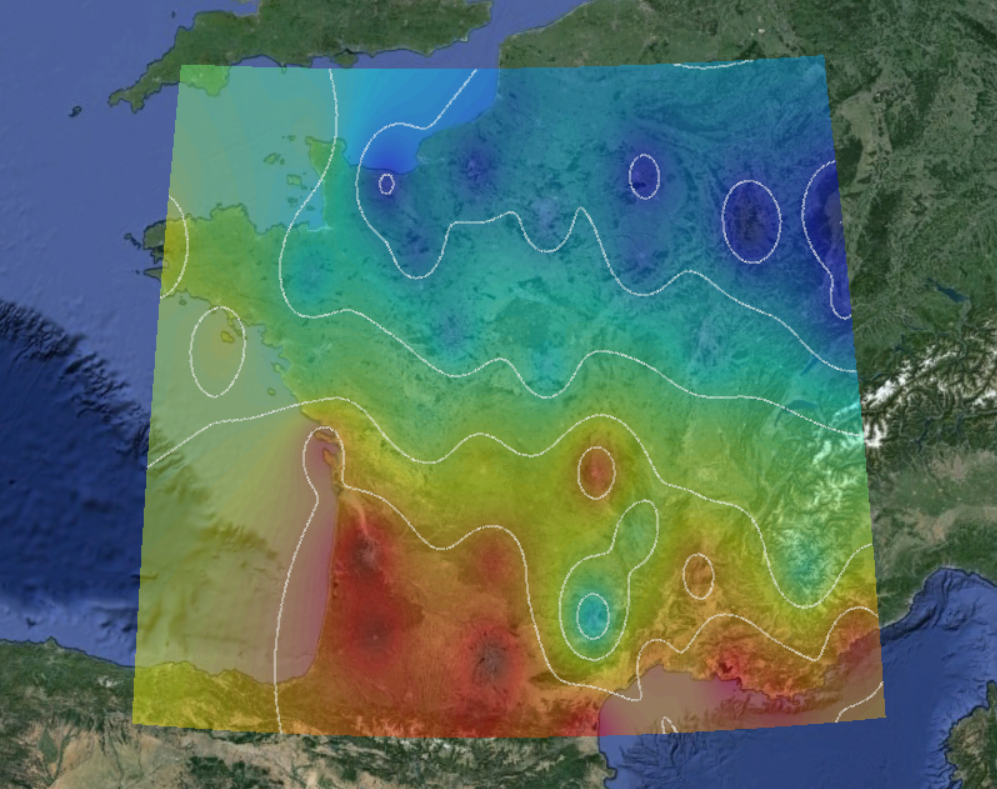
\includegraphics[width=0.86\linewidth]{img/temperature.png}
		\caption{colormap and isolines of temperature}
	\end{minipage}%
	\begin{minipage}{.5\textwidth}
		\centering
		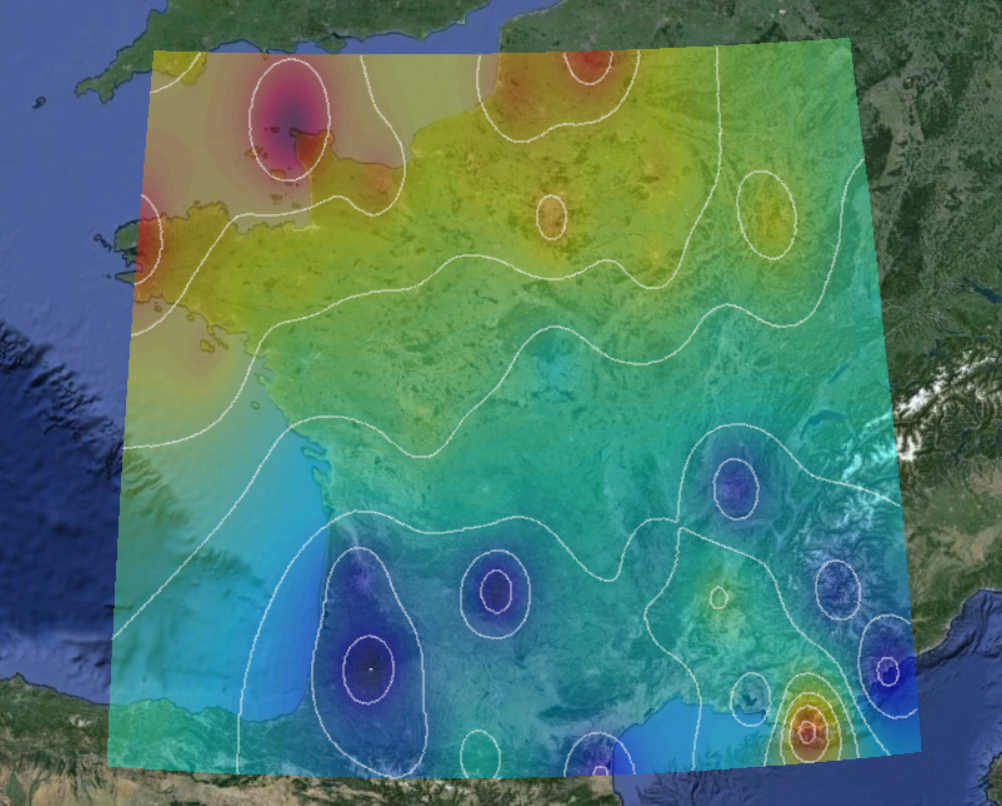
\includegraphics[width=0.86\linewidth]{img/wind.png}
		\caption{colormap and isolines of wind velocity}
	\end{minipage}
\end{figure}

\lstlistoflistings

\listoffigures

\begin{thebibliography}{5}

\bibitem{shepard}
  Shepard, D.,
  \emph{A two-dimensional interpolation function for irregularly-spaced data}.
  ACM '68 Proceedings of the 1968 23rd ACM national conference, New York
  1968.
  
\bibitem{hardy}
  Hardy, R.,
  \emph{Multiquadric equations of topography and other irregular surfaces}.
  J. Geophys. Res., 76 (8),
  1971.
  
\bibitem{micchelli}
  Micchelli, C.,
  \emph{Interpolation of scattered data: Distance matrices and conditionally positive definite functions}.
  Constr. Approx., 2,
  1986.

\end{thebibliography}

\end{document}